\section{Regex Engines}
Group 4, 5 and 6 need to explain what the difference is about text-directed and regex-directed engine for regex.
source : [[http://www.regular-expressions.info/engine.html]]

\subsection{technologies}
There are two underlying technologies commonly used to implement a regex match 
engine: regex-directed NFA (Nondeterministic Finite Automation) and 
text-directed DFA (Deterministic Finite Automation). Of the two types of 
engines, “NFA” is more commonly used. Popular programming languages like Python, Ruby 
and PHP use the formatting provided by NFA engines. DFA engines are more commonly seen 
in tools like egrep and awk. grep even employs a hybrid engine model where situationally 
the type of engine is switched around.

\subsection{matching}
A NFA must try every possible permutation of the regex before it can conclude that there's 
no match. A DFA finds the longest leftmost match. A Traditional NFA might also, or it might find something 
else. Any individual engine always treats the same regex/text combination in the 
same way, so in that sense, the regex isn't random, but other NFA engines may 
decide to do slightly different things. DFA Text-Directed Engines find the longest 
possible match. They are considered to be consistent and very fast due to their 
ability to simultaneously parse portions of the regex. NFA Regex-Directed Engines 
must work through a match. An NFA engine can support many things that a DFA cannot. 

Basically the regex-directed engine is way more flexible.
It contain options like:
\begin{itemize}
  \item lazy quantifiers (backtratracking of options) ex: <.+?>
  \item backreferences (Matches the same text as matched previously)
  \item atomic grouping (based to a capturing group but without backtracking) ex: a(?>bc|b)c
  \item possessive quantifiers (prevent the engine from trying all permutations)
\end{itemize}

During the course of an NFA match, the same character of the target 
might be checked by many different parts of the regex (or even by the same part, 
over and over). Even if a subexpression can match, it might have to be applied again 
(and again and again) as it works in concert with the rest of the regex to find a match. 
A local subexpression can fail or match, but you just never know about the overall match 
until you eventually work your way to the end of the regex. On the other hand, a DFA 
engine is deterministic: each character in the target is checked once (at most). When a 
character matches, you don't know yet if it will be part of the final match (it could be 
part of a possible match that doesn't pan out), but since the engine keeps track of all 
possible matches in parallel, it needs to be checked only once, period.

\begin{figure}[h]
	\centering
	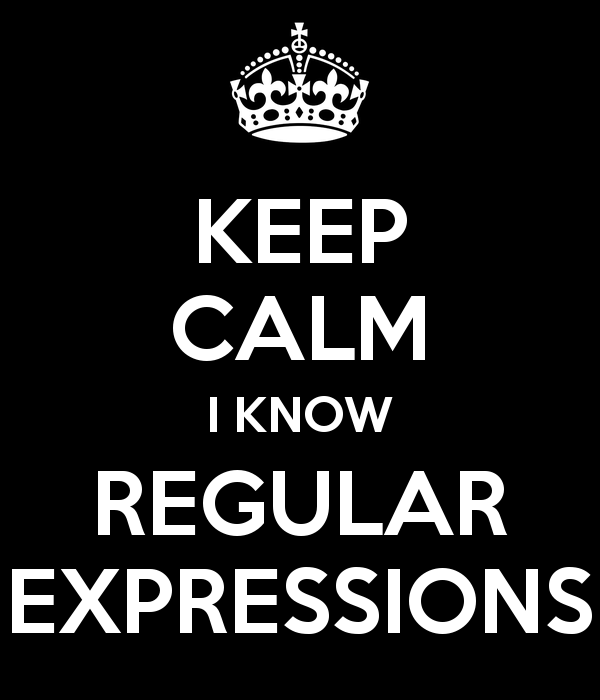
\includegraphics[width=100mm]{img/regex.png}
	\caption{I know Regex}
\end{figure}